\documentclass{xmgr}

\usepackage{float}
% minted listings
\usepackage{minted}
\usemintedstyle{trac}
\fvset{fontsize=\small}
\fvset{xleftmargin=2pt}

\usepackage{listings}
% "define" Scala
\usepackage{lstlang0}

% Default settings for code listings
\lstset{frame=tb,language=Scala,aboveskip=3mm,belowskip=3mm,showstringspaces=false,columns=flexible,basicstyle={\small\ttfamily}}

%\defaultfontfeatures{Scale=MatchLowercase}
%\setmainfont[Numbers=OldStyle,Ligatures=TeX]{Minion Pro}
%\setsansfont[Numbers=OldStyle,Ligatures=TeX]{Myriad Pro}
% for fontspec version < 2.0
\setmainfont[Numbers=OldStyle,Mapping=tex-text]{Minion Pro}
\setsansfont[Numbers=OldStyle,Mapping=tex-text]{Myriad Pro}
%\setmonofont[Scale=0.75]{Monaco}

% Opcjonalnie identyfikator dokumentu 
% drukowany tylko z~włączoną opcją 'brudnopis':
\wersja   {wersja wstępna [\ymdtoday]}

\author   {Mateusz Szygenda}
\nralbumu {186\,436}
\email    {mateusz.szygenda@gmail.com}

\title    {Wykorzystanie baz grafowych w~języku Scala}
\date     {2014}
\miejsce  {Gdańsk}

\opiekun  {dr Wiesław Pawłowski}

% dodatkowe polecenia
%\renewcommand{\filename}[1]{\texttt{#1}}


\begin{document}
\nocite{*}

\begin{abstract}
Praca ma na celu zademonstrowanie sposobu w~jaki można wykorzystać bazy grafowe w~nowoczesnych językach takich jak Scala. Jako część programistyczna powstało narzędzie NeoDSL. Jest to mini-język pozwalający na zapisywanie zapytań baz grafowych wprost w~kodzie programów pisanych w~języku Scala.
\end{abstract}
\keywords{Scala, Neo4j, DSL, języki dziedzinowe, bazy grafowe}

% tytuł i~spis treści
\maketitle

%
% wstęp
\introduction

W ostatnich latach można było zaobserwować pojawienie się wielu baz danych zrywających z~niepodzielnie dotychczas panującym paradygmatem baz relacyjnych. Mowa tutaj o~bazach nazywanych wspólnym hasłem ,,NoSQL" takich jak dokumentowa MongoDB czy też grafowa Neo4j. W~określonych warunkach oferują one dużo większą wydajność niż bazy relacyjne. Oczywiście odbywa się to pewnym kosztem. W~przypadku baz dokumentowych jest to zerwanie z~normalizacją oraz transakcyjnością lub z~całkowitą zmianą paradygmatu jak ma to miejsce w~przypadku baz grafowych. Poszukiwanie wydajniejszych rozwiązań do składowania danych ma oczywiście swoją przyczynę. Jest to mianowicie fakt iż współczesne aplikacje internetowe muszą obsługiwać miliony użytkowników w~czasie rzeczywistym. Baza danych która jest niejednokrotnie głównym elementem układanki musi oczywiście sprostać tym wymaganiom. Okazuje się jednak, że w~przypadku danych w~których rekordy są ze sobą ściśle powiązane wieloma zależnościami bazy relacyjne mogą nie być rozwiązaniem optymalnym. Wynika to ze sposobu w~jaki zależności te są modelowane w~bazach relacyjnych. Wykorzystywany mianowicie jest mechanizm kluczy obcych, natomiast na poziomie języka zapytań wykonywany jest iloczyn kartezjański co przy dużej ilości danych i~kilku relacjach może być bardzo kosztowne -- zarówno pod względem czasu, jak i~wykorzystywanej pamięci. Z~punktu widzenia użytkownika jest całkowicie nie do zaakceptowania by obsłużenie jego żądania zajmowało czas rzędu kilkunastu sekund lub nawet minut (por. \ref{fig:mysqlvsneo4j_results}). Potrzeba zatem wydajnego mechanizmu, który byłby w~stanie spełnić rygorystyczne wymogi wydajnościowe oraz dobrze radzić sobie z~danymi powiązanymi wieloma relacjami. Odpowiedzią są bazy grafowe, które do reprezentowania danych stosują strukturę grafu. Jak zostanie to wyjaśnione  w~dalszych rozdziałach ma to znaczący wpływ na wydajność i~sposób operowania na danych. Celem pracy było stworzenie narzędzia dla języka Scala pozwalającego na efektywne wykorzystanie jednej z~bardziej popularnych baz grafowych -- Neo4j. Język ten został wybrany ze względu na dostępność licznych mechanizmów ułatwiających definiowanie tzw. języków dziedzinowych (DSL).

\chapter{Bazy grafowe}

\section{Wstęp}

Z matematycznego punktu widzenia\cite{Szepietowski:2010:MD} graf to struktura składająca się ze zbioru wierzchołków oraz zbioru krawędzi. Krawędź reprezentuje połączenie pomiędzy dwoma wierzchołkami. W~przypadku gdy kierunek krawędzi jest istotny mówimy o~grafach skierowanych. Bazy grafowe wykorzystują właśnie tę strukturę reprezentowania wszystkich danych rozszerzając ją tylko w~nieznaczny sposób (np. dodając pojęcie nazwanych krawędzi). Pomimo faktu iż teoria grafów jest dziedziną niemłodą to same bazy grafowe są stosunkowo świeżym tworem. Jak wspomina autor bazy Neo4j, w~roku 1999 nie istniała praktycznie żadna baza grafowa mogąca być wykorzystana w~sposób produkcyjny \cite{Robinson:2013:GD}. Sposób w~jaki bazy grafowe prezentują dane implikuje odmienny sposób przeszukiwania i~operowania na zbiorze danych. Nie istnieje tutaj pojęcie tabeli znane z~baz relacyjnych takich jak MySQL, która narzucała by określoną strukturę. Zamiast tego mamy do czynienia z~wierzchołkami (nazywanymi w~dalszej części pracy zamiennie węzłami) które mogą zawierać dowolną liczbę pól prostych lub złożonych (jak ma to miejsce np. w~bazie OrientDB). Pod tym względem przypominają one bazy dokumentowe w~których również nie ma narzuconej struktury. W~odróżnieniu jednak zarówno od baz relacyjnych jak i~dokumentowych, w~bazach grafowych związki między obiektami są zapisywane za pomocą nazwanych i~skierowanych krawędzi. Pojedynczy węzeł może mieć dowolnie wiele krawędzi wychodzących jak i~wchodzących (w dalszej części pracy będziemy używać zamiennie terminu krawędź i~związek). Przeszukiwanie baz grafowych odbywa się poprzez definiowanie interesujących wzorców w~grafie. Dzięki efektywnym algorytmom przeszukiwania grafów taki sposób przechowywania danych ma znaczący wpływ na wydajność.

Aby dać czytelnikowi pogląd na to jak bardzo efektywne mogą być bazy grafowe w~porównaniu z~bazami relacyjnymi przedstawiony został eksperyment pochodzący z~książki ,,Neo4j In Action"\cite{neo4jinaction}. Ukazuje on porównanie wydajnościowe grafowej bazy Neo4j oraz MySQL dla analogicznej struktury danych. Poniższa ilustracja przedstawia prosty schemat bazy relacyjnej z~dwiema tabelami służącymi do przechowywania osób i~relacji ,,znajomości" między nimi.

\begin{figure}[H]
        \centering
	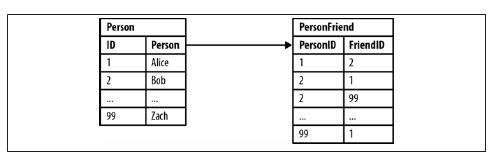
\includegraphics[scale=0.75]{images/relational-schema-friends.png}
	\caption{Schemat relacyjnej bazy przechowującej osoby i informacje o znajomych. Ilustracja z~książki ,,Graph Databases"\cite{Robinson:2013:GD}}
\end{figure}

Przykładowe zapytanie SQL do wyszukiwania znajomych znajomych osoby o~imieniu Alicja wygląda następująco.

\begin{listing}[H]
	\inputminted{sql}{listings/sql/relational-schema-friends-fof-query.sql}
	\caption{Zapytanie SQL do wydobycia znajomych znajomych Alicji. Przykład z~książki ,,Graph Databases"\cite{Robinson:2013:GD}}
\end{listing}

\newpage
Wraz ze wzrostem głębokości przeszukiwanych powiązań (znajomi znajomych znajomych itd.) potrzebne jest skorzystanie z~kolejnych instrukcji \texttt{JOIN}. Poniżej przedstawiona została tabela zestawiająca czasy wykonania zapytań wraz ze wzrostem ,,głębokości" zapytania dla zbioru 1 000 000 rekordów.

\begin{table}[H]
    \centering
    \begin{tabular}{|l|l|l|l|}
      \hline 
      \textbf{Głębokość} & \textbf{Czas (s) -- MySQL} & \textbf{Czas (s) -- Neo4j} & \textbf{Ilość wyników} \\
      \hline
      2 & 0.016 & 0.01 & {~}2500 \\
      3 & 30.267 & 0.168 & {~}110000 \\
      4 & 1543.505 & 1.359 & {~}600000 \\
      5 & Nieukończone & 2.132 & {~}800000 \\
      \hline
   \end{tabular} 
    \caption{Czas wykonania zapytań wraz ze wzrostem głębokości zapytania. Eksperyment z~książki ,,Neo4j in action"\cite{neo4jinaction}}
    \label{fig:mysqlvsneo4j_results}
\end{table}

Jak można zaobserwować na powyższym przykładzie, różnica pomiędzy MySQL i~Neo4j w~czasie wykonania zapytań dla głębokości trzy i~większej jest znacząca na korzyść tej drugiej. Wynika to z~odmiennego sposobu w~jaki odbywa się przeszukiwanie w~tych bazach. W~przypadku baz relacyjnych wzrost ,,głębokości" zapytania wiąże się z~tworzeniem kolejnego iloczynu kartezjańskiego. Dopiero po jego utworzeniu dane nieistotne są odrzucane z~wyników. W~przypadku dużego zbioru danych takie działanie odbija się na wydajności całego zapytania. Inaczej sytuacja wygląda w~bazach grafowych w~których rozpatrywane są wyłącznie węzły związane ze sobą krawędziami (jest to tzw. lokalność operacji).

\section{Rodzaje baz grafowych}

\subsection{Bazy z~relacyjnym magazynem danych}

Rozróżniamy dwa główne rodzaje baz grafowych. Pierwszym z~nich są bazy które pozwalają operować na przechowywanych danych jak na grafach, mających jednak odmienny sposób składowania danych. Popularnym rozwiązaniem jest np. przechowywanie struktury grafowej w~bazach relacyjnych. Niestety takie rozwiązanie nie pozwala na pełne wykorzystanie potencjału drzemiącego w~przechowywaniu danych w~postaci grafów. Przykładem takiej bazy jest FlockDB\cite{flockdb} która znajduje zastosowanie w~popularnym serwisie społecznościowym Twitter. Ze względu na małą uniwersalność tego typu rozwiązań (zazwyczaj są one dostosowane do konkretnego przypadku użycia) nie będą one omawiane w~tej pracy.

\subsection{Bazy z~grafowym magazynem danych}
Drugim rodzajem baz grafowych są natywne bazy grafowe które nie tylko przedstawiają dane w~formie grafów ale również wykorzystują strukturę grafów do ich składowania. Zaletą takiego podejścia jest to iż przeszukiwanie może okazać się o~wiele wydajniejsze niż równoważne zapytanie do bazy z~relacyjnym magazynem danych. Powodem tego jest lokalność operacji wykonywanych na grafie. W~odróżnieniu od baz relacyjnych gdzie by wyszukać dane powiązane pewną relacją wymagane jest wykonanie iloczynu kartezjańskiego na całych zbiorach danych. W~przypadku ogromnej liczby rekordów taka operacja może okazać się wielce niewydajna. W~przypadku baz grafowych nie ma potrzeby odwiedzania wszystkich danych bowiem poruszamy się tylko w~obrębie obiektów w~bezpośredni sposób związanych ze sobą krawędziami. Przykładem takiej bazy jest Neo4j której została poświęcona znaczna część tej pracy.

\chapter{Neo4j}

Neo4j jest natywną bazą grafową napisaną w~języku Java. Pozwala ona na przechowywanie węzłów jak i~krawędzi wraz z~polami typów prostych takimi jak napisy czy liczby. W~implementacji zostało zastosowanych wiele mechanizmów mających na celu osiągnięcie jak najlepszej wydajności przy przeszukiwaniu grafów. Warto tutaj wymienić chociażby sposób w~jaki zapisywana jest informacja o~krawędziach wychodzących z~wierzchołka. Otóż, aby odczytać listę krawędzi dla danego wierzchołka nie ma potrzeby korzystania z~żadnego pośredniczącego indeksu, informację tę można odczytać bezpośrednio w~jednym kroku (ang. Index-Free Adjacency\cite[s.~5]{Robinson:2013:GD}). Wierzchołki i~krawędzie są natomiast zapisywane w~plikach w~których każdy rekord jest stałego rozmiaru. Pozwala to na bardzo szybkie odczytywanie danych bez konieczności przeglądania pliku w~celu odnalezienia właściwego rekordu (wystarczy pomnożyć rozmiar rekordu krawędzi bądź węzła przez jego identyfikator by uzyskać lokalizację w~pliku).

Neo4j jest wydajną i~jedną z~bardziej popularnych baz grafowych. Z~tego powodu została ona wybrana do implementacji narzędzia będącego przedmiotem niniejszej pracy.

\section{Język Cypher}
Cypher jest językiem zapytań stworzonym specjalnie na potrzeby Neo4j pozwalającym w~sposób deklaratywny przeszukiwać oraz aktualizować bazę grafową. Podobnie jak SQL jest to stosunkowo łatwy w~analizie język który oferuje duże możliwości. Podrozdział ten ma na celu zaznajomienie czytelnika z~podstawami składni i~sposobem w~jaki operuje się za jego pomocą na danych w~bazach grafowych.

\newpage

\subsection{Przeszukiwanie grafu}

Najistotniejszą funkcjonalnością baz danych jest możliwość przeszukiwania zbioru rekordów. W~języku Cypher, zapytanie służące do odczytywania informacji składa się z~trzech podstawowych części.

Sekcja \texttt{START} pozwala na ustalenie węzłów startowych od których zacznie się przeszukiwanie grafu. Wierzchołki można wydobyć na podstawie ich wewnętrznego identyfikatora lub z~wykorzystaniem przygotowanego wcześniej indeksu. Sekcja ta do wersji 1.9 była obligatoryjna i~mimo iż w~nowych wersjach możliwe jest jej całkowite pominięcie zalecane jest aby zawsze określać węzły startowe\footnote{Brak określenia węzłów startowych może negatywnie wpłynąć na wydajność, gdyż do później zdefiniowanego wzorca będzie dopasowany każdy węzeł znajdujący się w~bazie danych}. Poniższy przykład ilustruje sposób w~jaki można określić wierzchołki początkowe. Zmiennej \texttt{comment} przypisany jest węzeł o~wewnętrznym identyfikatorze równym 1, natomiast \texttt{john} będzie wskazywał na węzły znajdujące się w~indeksie nazwanym \texttt{nameIndex} oraz zawierające pole \texttt{name} o~wartości równej ,,John".

\inputminted{cypher}{listings/cypher/start-section.cypher}

Sekcja \texttt{MATCH} jest główną częścią zapytania, pozwala ona bowiem określić interesujące nas wzorce w~grafie. Część ta jest swego rodzaju ,,odpowiednikiem" instrukcji \texttt{INNER JOIN} języka SQL, gdyż pozwala nam określić interesujące powiązania pomiędzy węzłami. Poniżej został zdefiniowany jeden wzorzec który pozwala wyszukać znajomych Johna ,,lubiących" komentarz wskazywany przez zmienną \texttt{comment}

\inputminted{cypher}{listings/cypher/match-section.cypher}

Ostatnim elementem zapytania jest sekcja \texttt{RETURN} służąca określania pól które mają zostać zwrócone jako wynik. W~poniższym przykładzie zwrócone zostanie pole \texttt{name} oraz wewnętrzny identyfikator węzłów dopasowanych do zmiennej \texttt{friend}.

\inputminted{cypher}{listings/cypher/return-section.cypher}

Pełne zapytanie zwraca identyfikator oraz pole \texttt{name} węzłów które są połączone krawędzią o~nazwie \texttt{KNOWS} z~obiektem \texttt{john} oraz krawędzią \texttt{LIKES} -- z~obiektem o~identyfikatorze równym {1}. Poruszając się w~domenie sieci społecznościowej zapytanie zwraca znajomych użytkownika ,,John" którzy polubili komentarz o~identyfikatorze {1}.

\inputminted{cypher}{listings/cypher/sample-query.cypher}

\subsection{Modyfikacja danych}

Język Cypher pozwala również na aktualizację danych w~grafie. Podobnie jak w~przypadku zapytania służącego do przeszukiwania grafu wyrażenie składa się kilku części.

Pierwszą z~nich ponownie jest sekcja \texttt{START}, która pozwala na wybranie węzłów zakotwiczających tworzony wzorzec w~strukturze grafu. Jest ona opcjonalna jeśli zamierzamy utworzyć graf niepowiązany z~istniejącymi już wierzchołkami.

\inputminted{cypher}{listings/cypher/start-section.cypher}

Kolejną sekcją jest \texttt{CREATE} której składnia jest podobna do sekcji \texttt{MATCH}. W~przeciwieństwie jednak do \texttt{MATCH} pozwala ona na tworzenie powiązań oraz węzłów w~grafie. W~poniższym przykładzie zostanie utworzony węzeł \texttt{newFriend} o~polu \texttt{name} równym wartości ,,New friend" oraz krawędź \texttt{KNOWS} łącząca wierzchołek wskazywany przez zmienną \texttt{john} z~nowo utworzonym węzłem.

\inputminted{cypher}{listings/cypher/create-section.cypher}

Ostatnim elementem jest wykorzystana już wcześniej sekcja RETURN która pozwala na zwrócenie informacji o~nowo-utworzonych obiektach, np. ich identyfikatory.

\inputminted{cypher}{listings/cypher/return-section-2.cypher}

Pełne zapytanie wstawiające do grafu nowy obiekt o~polu \texttt{name} równym ,,New Friend" i~łączące go z~obiektami \texttt{john} oraz \texttt{comment} wygląda następująco

\inputminted{cypher}{listings/cypher/sample-create-query.cypher}

\section{Programistyczne sposoby dostępu do Neo4j}

Neo4j udostępnia kilka odmiennych sposobów dostępu do bazy. Rozdział ten ma na celu przedstawienie każdego z~nich.

\subsection{Java Core API -- Embedded mode}

Jedną z~możliwości jest skorzystanie z~tzw. Java Core API czyli zestawu klas i~interfejsów dostępnych dla języka Java. Udostępnionych został szereg mechanizmów pozwalających na operowanie na węzłach i~związkach w~sposób bezpośredni.

\medskip\noindent Do rozpoczęcia pracy potrzebna jest instancja bazy. Można ją utworzyć w~następujący sposób.

\inputminted{java}{listings/java/neo4j-core-api-dbcreate.java}

Powyższy fragment kodu powinien utworzyć instancję bazy pod ścieżką ,,/tmp/neo4j".

Z wykorzystaniem tak utworzonej bazy danych możliwe jest wstawianie oraz odczytywanie węzłów i~krawędzi. Oto fragment kodu demonstrujący podstawowe operacje.

\newpage

\inputminted{java}{listings/java/neo4j-core-api-use.java}

Oczywistą wadą jest fakt, że do wykorzystania tego mechanizmu potrzebna jest lokalna instancja bazy danych.

\subsection{Traversal Framework API}

Uzupełnieniem poprzedniego mechanizmu jest tzw. Traversal Framework który pozwala w~prosty sposób na definiowanie algorytmu przechodzenia po grafie. Podstawowym interfejsem jest \texttt{TraversalDescription}, który służy do określania zasad przechodzenia grafu. Oczywiście nikt nie wymaga od programisty by tworzył złożoną implementację algorytmu odwiedzania grafu. Neo4j udostępnia szereg standardowych metod służących do poruszania się po krawędziach określonego typu oraz do komponowania tychże metod ze sobą.

Poniżej przedstawiony został przykład w~jaki sposób można zdefiniować ,,opis" metody wyszukiwania węzłów połączonych w~sposób bezpośredni krawędzią ,,KNOWS" z~wierzchołkiem \texttt{john}

\inputminted{java}{listings/java/neo4j-traversal-api-knows.java}

\subsection{REST mode}

Ostatnim ze sposobów dostępu do bazy Neo4j jest użycie serwisu REST--owego. W~tym trybie korzystając z~protokołu HTTP odwołujemy się do usług pozwalających między innymi na wykonywanie poleceń języka Cypher. Niewątpliwą zaletą tego podejścia jest niezależność od platformy. Z~wystawionego serwisu można skorzystać z~poziomu praktycznie każdego języka programowania. Dodatkowo, w~odróżnieniu od embedded mode nie ma potrzeby aby baza danych znajdowała się na tym samym serwerze co aplikacja.

Usługa serwera udostępnia standardowe akcje służące do tworzenia, wyszukiwania węzłów oraz krawędzi czy też uruchamiania zapytań języka Cypher. Ze względu na swoją uniwersalność właśnie ten sposób dostępu do bazy danych został wykorzystany w~narzędziu powstałym w~ramach tej pracy.

Oto przykładowe żądanie zlecające wykonanie zapytania języka Cypher (wysłane z~wykorzystaniem narzędzia ,,curl")

\inputminted{bash}{listings/bash/neo4j-rest-cypher.sh}

\chapter{Język Scala}

Scala jest statycznie typowanym językiem programowania który łączy w~sobie idee programowania obiektowego oraz funkcyjnego. Połączenie tych dwóch paradygmatów było jednym ze środków do osiągnięcia głównego z~założeń twórców jakim było stworzenie języka, który jest skalowalny oraz zwięzły. Skalowalność w~tym przypadku polega na przystosowaniu języka do prostych zadań jak np. niewielkie skrypty oraz do ogromnych projektów jakie realizuje się w~językach typu Java czy C\#.

Do dyspozycji programisty zostało oddanych szereg mechanizmów pozwalających na ,,rozszerzanie" składni języka. Jednym z~nich jest np. możliwość definiowania metod zawierających w~nazwie symbole uchodzące w~innych językach za specjalne (takie jak \texttt{*}, \texttt{+}, \texttt{-} etc.). Pozwala to na definiowanie ,,operatorów" które w~innych językach takich jak Java są traktowane w~sposób szczególny. Scala jest tak elastycznym narzędziem iż pozwala nawet na definiowanie znanych struktur kontrolnych takich jak np. pętla \texttt{while}. Warto również wspomnieć o~niejawnym przekazywaniu parametrów i~wywoływaniu metod. Możliwe jest zdefiniowanie metody której jeden z~argumentów dostarczany jest w~sposób niejawny (bez wiedzy programisty) poprzez wyszukanie pasującego obiektu w~miejscu wywołania metody. Podobnie mechanizm działa w~przypadku niejawnych metod gdzie możliwe jest ich wykonanie w~sytuacji gdy typ przekazywanego wyrażenia jest niezgodny z~oczekiwanym.

Pomimo tego, że Scala jest językiem statycznie typowanym, nie wymaga od programisty jawnego określania typu w~każdej sytuacji. System inferencji typów jest na tyle rozbudowany iż w~wielu przypadkach możliwe jest całkowite pominięcie określania typów zmiennych. Jest to kolejna cecha poza wieloma innymi wpływająca na zwięzłość kodu pisanego w~tym języku.

Właśnie z~powodów zwięzłości oraz łatwości z~jaką możliwe jest rozszerzanie składni, Scala została wybrana do stworzenia języka dziedzinowego do obsługi baz grafowych.

\subsection{Programowanie funkcyjne}

Języki takie jak Java, C\# czy C++ są obiektowymi językami programowania opartymi na paradygmacie programowania imperatywnego. Zakłada on istnienie \textit{stanu} w~programie, który podlega ciągłej zmianie. Przeciwieństwem tego podejścia jest programowanie funkcyjne, w~którym nie istnieje stan, a~funkcje przekształcają dane wejściowe w~wyjściowe bez tzw. efektów ubocznych. Kolejną cechą języków funkcyjnych jest to iż funkcje są traktowane jak zwykłe wartości. Możliwe jest na przykład przekazywanie ich jako parametrów innych funkcji, w~identyczny sposób jak dzieje się to z~instancjami typów \texttt{String} czy \texttt{Integer}. Scala łączy te dwa odmienne podejścia dając programiście swobodę w~wyborze najbardziej odpowiedniego rozwiązania implementacyjnego.

\subsection{Podstawy składni}
Składnia Scali była inspirowana takimi językami jak C\# czy Java stąd doświadczonym programistom nie powinno sprawiać trudności czytanie kodu w~tyn języku. Oczywiście, jak zostało to już wspomniane, w~odróżnieniu od wspomnianych języków Scala wprowadza szereg usprawnień wpływających na zwięzłość pisanego kodu. Nie ma np. potrzeby kończenia każdej linii średnikiem czy jawnego określania typu każdej zmiennej (o ile system inferencji jest w~stanie go wyliczyć).

Istotną różnicą w~stosunku do Javy czy C\# wpływającą na czytelność kodu jest sposób w~jaki definiuje się zmienne czy parametry metod. Mianowicie, najpierw określa się ich nazwy a~w drugiej kolejności typ (który może być całkowicie pominięty jeśli da się go określić z~systemu inferencji). Taka kolejność umotywowana jest tym iż programista czytający kod bardziej zainteresowany jest nazwą aniżeli typem zmiennej. Poniżej kilka przykładowych deklaracji wartości i~zmiennych.

\newpage

\inputminted{scala}{listings/scala/val-var-declarations.scala}

Metody w~języku Scala definiuje się z~użyciem słowa kluczowego \texttt{def}. Podobnie jak w~przypadku zmiennych typ zwracanej wartości określany jest po zdefiniowaniu nazwy i~może być on całkowicie pominięty jeśli da się go określić z~ciała metody. Poniżej przykłady kilku funkcji.

\inputminted{scala}{listings/scala/functions-example.scala}

Klasy definiuje się z~użyciem słowa kluczowego \texttt{class} podobnie jak ma to miejsce w~Javie. To na co warto zwrócić uwagę, to fakt iż klasy języka Scala posiadają tzw. konstruktor główny. Jego parametry określa się bezpośrednio po nazwie klasy natomiast implementacja powinna być zawarta w~ciele klasy. W~ramach listy parametrów konstruktora głównego możliwe jest również zdefiniowanie pól składowych klasy z~użyciem słów kluczowych \texttt{val} lub \texttt{var} (służą one odpowiednio do deklarowania wartości lub zmiennych). Wszelkie przeciążone konstruktory (które definiuje się podobnie jak w~Javie) muszą skorzystać w~sposób pośredni lub bezpośredni z~konstruktora głównego.

Poniżej przedstawiona została prosta klasa Person w~języku Scala. W~konstruktorze głównym zdefiniowane zostały dwa pola składowe: \texttt{name} oraz \texttt{age}.

\inputminted{scala}{listings/scala/simple-class-person.scala}

Poza tym klasa zawiera jedną metodę \texttt{sayHello} która wyświetla komunikat.
Zdefiniowanej powyżej klasie odpowiada poniższy kod w~języku Java.

\inputminted{scala}{listings/java/simple-class-person.java}

\subsection{Pattern Matching}

Jednym z~bardziej istotnych mechanizmów języka niespotykanym w~takich językach jak Java jest tzw. Pattern Matching (dopasowywanie do wzorca). Pozwala on na definiowanie specjalnych klas (ang. Case Classes) które można dopasowywać i~docierać do ich składowych z~wykorzystaniem dedykowanej do tego celu składni. Przypomina to trochę instrukcję \texttt{switch} o~dużo bardziej zaawansowanym działaniu. Oto przykład użycia tego mechanizmu do wyświetlenia wartości przechowywanych w~liściach struktury drzewa reprezentowanej właśnie przy pomocy tzw. case classes.
\newpage
\inputminted{scala}{listings/scala/pattern-matching-trees.scala}

W powyższym przykładzie zdefiniowana została cecha\footnote{W Scali cecha (ang. trait) to mieszanka koncepcji interfejsu oraz klasy abstrakcyjnej. Mogą one posiadać zarówno metody abstrakcyjne jak i~konkretne implementacje.} drzewa (ang. Tree) oraz podklasy liścia (ang. Leaf) przechowującego wartości typu \texttt{Int} i~węzła (ang. Node) posiadającego dwóch potomków. Metoda \texttt{showTree} zdefiniowana w~obiekcie \texttt{TreeProrgram} dopasowuje przekazany argument do wzorców liścia i~węzła. W~ramach tego dopasowania składowe klas zostają przypisane do identyfikatorów \texttt{left}, \texttt{right} oraz \texttt{value}. W~zależności od przekazanego argumentu wywołany zostanie odpowiedni blok kodu.

Pattern matching znajduje zastosowanie w~NeoDSL chociażby na etapie serializacji struktury zapytań do języka Cypher.

\chapter{Dostęp do baz danych z~wykorzystaniem DSL}

Wszystkie bazy danych udostępniają pewien natywny interfejs do manipulacji na przechowywanych rekordach. W~przypadku baz relacyjnych mamy do dyspozycji odpowiedni dialekt SQL. O~ile np. sam język SQL jest prostym w~użyciu narzędziem to rzadko kiedy z~poziomu tworzonego programu chcemy korzystać z~niego w~sposób bezpośredni. Potrzebna jest pewna warstwa abstrakcji która ukryje przed programistą różnice w~implementacji SQLa w~różnych bazach relacyjnych jak i~uchroni przed typowymi błędami takimi jak nie oczyszczanie danych pochodzących od użytkownika (prowadzących np. do ataków SQL Injection). Rozwiązaniem tego problemu są tzw. mappery bazodanowe takie jak Hibernate. Udostępniają one mechanizmy które pozwalają na zdefiniowanie powiązania pomiędzy klasami programu a~tabelami/kolekcjami w~bazie danych. Narzędzia te zajmują się tłumaczeniem wywołań odpowiednich metod na zapytania języka obsługiwanego przez daną bazę. Oprócz tego zamiast generycznych obiektów reprezentujących wyniki zapytań zwracają one instancje klas, które reprezentują poszczególne rekordy (np. instancje klas typu \texttt{Osoba}, \texttt{Komentarz}).

Alternatywą dla klasycznych rozwiązań typu Hibernate są języki dziedzinowe (ang. Domain Specific Language -- w~skrócie DSL)  pozwalające w~pewnym uproszczeniu na zapisywanie zapytań języka bazy danych wprost w~kodzie programu. Tak budowane zapytania są zwykłymi wywołaniami metod danego języka stąd są automatycznie walidowane na etapie kompilacji.

Rozdział ten ma na celu przedstawienie istniejących rozwiązań dla baz relacyjnych jak i~NoSQL będących inspiracją dla narzędzia NeoDSL stworzonego w~ramach tej pracy.

\newpage

\section{Bazy SQL}

\subsection{Squeryl}

Sztandarowym przykładem DSLa bazodanowego dla języka Scala jest projekt Squeryl. Umożliwia on definiowanie struktury bazy danych w~kodzie programu a~następnie budowanie zapytań z~jej wykorzystaniem.

Pierwszym etapem w~przypadku narzędzia Squeryl jest stworzenie odwzorowania struktury bazy danych. Definiuje się je z~wykorzystaniem zwykłych klas języka Scala oraz specjalnej cechy \texttt{Schema}. Przykładowa struktura (zaczerpnięta z~dokumentacji Squeryla\cite{squeryl_schemadefinition}) przedstawiona jest poniżej.

\inputminted{scala}{listings/scala/squeryl-schema.scala}

Powyższa struktura odwzorowuje bardzo prostą bazę danych z~jedną tabelą \texttt{Song} służącą do przechowywania informacji o~utworach muzycznych. Z~wykorzystaniem tak zdefiniowanych klas możliwe jest budowanie zapytań. Przykładem może być zapytanie

\inputminted{scala}{listings/scala/squeryl-query.scala}

\noindent służące do wyszukiwania piosenek, które w~tytule zawierają słowo ,,funk". Jest ono równoważne poniższemu zapytaniu w~języku SQL.

\inputminted{sql}{listings/sql/squeryl-query.sql}

Zastosowanie języka dziedzinowego pozwala w~pełniejszy sposób wykorzystać możliwości języka bazy danych przy jednoczesnym zachowaniu zalet rozwiązań typu Hibernate (tj. odwzorowywanie wyników na obiekty oraz kontrola wyrażeń na etapie kompilacji).

\section{Bazy NoSQL}

MongoDB jest jedną z~popularniejszych baz dokumentowych. Pozwala ona na przechowywanie tzw. dokumentów tj. rekordów nie mających ustalonego z~góry schematu. Dodatkowo poza polami prostymi takimi jak liczby czy napisy dozwolone jest zagnieżdżanie w~sobie złożonych obiektów. W~określonych sytuacjach MongoDB oferuje dużą lepszą wydajność w~porównaniu z~bazami relacyjnymi. Odbywa się to jednak kosztem zerwania z~normalizacją i~brakiem transakcyjności.

\subsection{Rogue}

Jedną z~bibliotek do obsługi MongoDB z~poziomu języka Scala jest Rogue. Podobnie jak Squeryl udostępnia ona DSL służący do budowania zapytań. Oto przykładowa klasa modelu składowanego w~MongoDB.

\inputminted{scala}{listings/scala/rogue-model.scala}

Jak można zauważyć na powyższym przykładzie, do definiowania pól konieczne jest tworzenie obiektów rozszerzających cechę \texttt{Field}. Skutkuje to tym iż do osiągnięcia takich samych rezultatów jak w~przypadku Squeryl-a potrzebne jest napisanie nieco dłuższego kodu. Zaprezentowane rozwiązanie ma jednak tę zaletę, że dzięki specjalnym typom jak np. \texttt{LongField} dużo łatwiejsze stało się tworzenie DSL-a który nie musi zajmować się obsługą typów wbudowanych w~język Scala.

\medskip\noindent Przykładowe zapytanie przedstawione jest poniżej.

\inputminted{scala}{listings/scala/rogue-query.scala}

\chapter{DSL do baz grafowych}

W celu zaprezentowania jednego ze sposobów w~jaki można wykorzystać bazy grafowe w~nowoczesnych językach jak Scala powstało narzędzie NeoDSL\footnote{Dostępne pod adresem \url{https://github.com/mszygenda/neodsl}}. Jest to DSL służący do obsługi baz grafowych.
Obecnie jedynym obsługiwanym silnikiem bazy danych jest Neo4j. Jednak nic nie stoi na przeszkodzie aby w~przyszłości została dodana obsługa innych baz. Wynika to z~faktu, że warstwa zajmująca się wykonywaniem zapytań została ujęta w~sposób abstrakcyjny.

Podobnie jak w~bibliotece Squeryl, w~NeoDSL przed tworzeniem jakichkolwiek zapytań trzeba zdefiniować strukturę bazy danych. Inaczej jednak niż w~przypadku Squeryl-a, odbywa się to wyłącznie na poziomie klas domenowych. Nie ma potrzeby tworzenia jednego specjalnego obiektu skupiającego w~sobie wszystkie powiązania. Dzięki określonej strukturze możliwe jest budowanie silnie typowanych wzorców i~całych zapytań. Jest to niewątpliwą zaletą w~stosunku do ,,ręcznego" pisania zapytań języka Cypher. Oczywiście wszystko będzie odpowiadało strukturze bazy pod warunkiem, że model został poprawnie zdefiniowany. Przypomnijmy, że w~bazach takich jak Neo4j nie istnieje pojęcie schematu i~nie ma z~góry określonej struktury. To programista lub narzędzie do obsługi bazy musi zapewnić spójność w~tym aspekcie.

\section{Definiowanie modelu}

Pierwszym krokiem jaki należy wykonać przed definiowaniem zapytań jest utworzenie modelu (tj. zbioru klas) odpowiadającego jakiemuś fragmentowi rzeczywistości, który opisujemy i~przechowujemy w~bazie danych. Neodsl udostępnia mechanizmy pomocnicze, które pozwalają na szybkie odwzorowanie węzłów oraz powiązań między nimi.

\newpage

\subsection{Klasa \texttt{DomainObject}}

Wszystkie klasy domenowe powinny rozszerzać \texttt{DomainObject}, która dostarcza narzędziu niezbędnych informacji do działania. Jest to klasa generyczna\footnote{Klasy generyczne  przyjmują dodatkowe parametry będące typami}, która wymaga określenia typu klasy, którą definiuje programista (konieczność przekazywania typu definiowanej klasy jest technicznym szczegółem, który wymagany jest do prawidłowego funkcjonowania narzędzia). 

\subsection{Krawędzie}

Do określania krawędzi wchodzących, wychodzących i~bez określonego kierunku węzłów danego typu służą metody odziedziczone z~klasy \texttt{DomainObject}, odpowiednio:  \texttt{<--}, \texttt{-->}, \texttt{--}\footnote{Scala pozwala na definiowanie operatorów składających się ze znaków uchodzących w~innych językach za specjalne. Odpowiadają one zwykłym metodom.}. Przyjmują one parametr będący typem spodziewanych węzłów po drugiej stronie krawędzi oraz argument służący do określania jej nazwy. Aby móc w~sensowny sposób budować zapytania, wartości zwracane przez wspomniane metody powinny zostać zapisane w~polach składowych klasy. Oto przykład w~jaki można zdefiniować krawędź o~nazwie ,,KNOWS" wychodzącą do obiektów typu \texttt{Person}.

\inputminted{scala}{listings/scala/dsl/simple-relation.scala}

\subsection{Przykład modelu}

Rozpatrzmy przykładową klasę domenową reprezentującą osobę. Zawiera ona pola \texttt{name} oraz \texttt{surname} odpowiadające imieniu i~nazwisku oraz pola definiujące krawędzie wychodzące z~węzłów tego typu. Jest to pole \texttt{knows}, które definiuje krawędź wychodzącą do obiektów typu \texttt{Person} oraz \texttt{wrote} -- reprezentujące związek pomiędzy \texttt{Person} a~obiektami typu \texttt{Comment} (w klasie \texttt{Comment} zdefiniowane jest odbicie symetryczne tego związku).

\newpage

\inputminted{scala}{listings/scala/dsl/sample-model.scala}

\section{Budowanie wzorców}

Zapytania w~bazach grafowych skupiają się na wyszukiwaniu określonych wzorców. Z~tego powodu główny nacisk w~kwestii zwięzłości tworzonego DSLa został położony właśnie na tej części.

\subsection{Podstawowa struktura -- \texttt{PatternTriple}}
Podstawową strukturą służącą do reprezentacji wzorców jest klasa \texttt{PatternTriple}. Jak sugeruje jej nazwa, składa się ona z~trzech elementów. Są to kolejno: węzeł początkowy, krawędź z~określonym kierunkiem oraz tzw. ,,ogon" wzorca. Wspomniany ,,ogon" może być zarówno pojedynczym węzłem jak i~kolejną instancją \texttt{PatternTriple}. Taka struktura pozwala na budowanie w~sposób rekurencyjny dowolnie długich wzorców. Warto również dodać iż klasa \texttt{PatternTriple} jest generyczna i~posiada z~góry określone typy węzłów jakie mogą pojawiać się w~dalszej części wzorca. Niemożliwe jest zatem utworzenie instancji wzorca, w~której zachodziłaby niezgodność typów (o to zadba kompilator języka Scala).

\subsection{Budowniczy wzorców -- \texttt{PatternBuilder}}
Aby uprościć budowanie trójek wzorca została przygotowana klasa \texttt{PatternBuilder} (nazywana dalej ,,budowniczym"), która jak sugeruje jej nazwa służy do budowania wzorców. Udostępnia ona szereg metod pomocniczych pozwalających na budowanie i~rozszerzanie istniejących instancji \texttt{PatternTriple}. Tworzenie instancji budowniczego jest niezwykle proste i~odbywa się na etapie definiowania klas domenowych, instancje klasy PatternBuilder zwracane są przez metody \texttt{-->}, \texttt{<--}, \texttt{--}.

Rozważmy przykładowe złożenie kilku wzorców. Wykorzystuje ono została tutaj zaprezentowaną wcześniej strukturę sieci społecznościowej. Pojawiające się poniżej zmienne \texttt{john}, \texttt{friend}, \texttt{matthew} są instancjami typu \texttt{Person} podczas gdy \texttt{wiseComment} jest obiektem typu \texttt{Comment}.

\inputminted{scala}{listings/scala/dsl/patterns/functional-example-1.scala}

Wartością powyższego wyrażenia jest instancja tzw. złożenia wzorców, mamy tutaj bowiem do czynienia z~trzema wzorcami połączonymi operatorem logicznym \texttt{and}. Wzorzec ten odpowiada poniższej sekcji \texttt{MATCH} języka Cypher.

\inputminted{cypher}{listings/cypher/patterns-dsl-example.cypher}

\section{Nakładanie warunków na wyniki zapytań}

Ważnym aspektem przy przeszukiwaniu baz danych jest możliwość nakładania ograniczeń na zwracane wyniki. Założeniem projektu było aby dało się wyrażać warunki logiczne bez potrzeby wprowadzania nowej składni innej niż ta, dostarczana przez sam język Scala. Oto przykład demonstrujący w~jaki sposób można nakładać warunki na zapytania w~NeoDSL.

\inputminted{scala}{listings/scala/dsl/query-with-simple-condition.scala}

Aby osiągnąć ten cel potrzebny okazał się mechanizm pozwalający na analizę wyrażeń typu \texttt{Boolean}. W~języku Scala zadanie to może być zrealizowane z~wykorzystaniem tzw. makr. 
Dzięki nim, możliwa jest transformacja wyrażenia typu \texttt{Boolean} na strukturę rozpoznawaną przez NeoDSL, która w~efekcie końcowym zamieniana jest na zapytanie języka Cypher.

\subsection{Makra}

Makra są eksperymentalną funkcjonalnością języka Scala wprowadzoną w~wersji 2.10.0. Są one, podobnie jak w~przypadku makr znanych z~języka C, wykonywane podczas etapu kompilacji jednak dają o~wiele więcej możliwości. Najważniejszą różnicą w~stosunku do wspomnianego C jest fakt, że makra języka Scala nie wymagają stosowania żadnego specyficznego dla tego typu zadań mini-języka. Zamiast tego, mogą być pisane w~języku Scala. Co więcej nie ograniczają się one do prostej zamiany tekstu w~kodzie programu jak to bywa w~przypadku innych języków, ale pozwalają na modyfikację drzewa składniowego. Oczywiście jest to dużo bardziej zaawansowany mechanizm i~jego właściwe wykorzystanie jest bardziej skomplikowane, niemniej w~zamian otrzymujemy bardzo potężne narzędzie.

Samo definiowanie makra jest stosunkowo proste. Wystarczy utworzyć obiekt\footnote{W Scali istnieje dedykowana instrukcja do tworzenia pojedynczej instancji obiektu, natomiast w~językach takich jak Java realizowane jest to za pomocą wzorca Singleton} z~dowolnie nazwaną metodą która docelowo ma służyć do wykonywania makra. W~przeciwieństwie do zwykłych metod, nie powinna ona zawierać ciała, a~jedynie słowo kluczowe \texttt{macro} wraz z~nazwą metody która implementuje dane makro. Najbardziej interesującym elementem jest właśnie metoda implementująca makro. Ma ona dwie listy parametrów. Pierwsza z~nich zawiera jeden parametr tzw. kontekst (typu \texttt{Context}), który udostępnia niezbędne metody do modyfikacji kodu. Druga --  drzewa składniowe wyrażeń jakie zostały przekazane do makra w~postaci argumentów. Zwracaną wartością jest drzewo składniowe które zostanie wstawione w~miejscu wywołania makra. Mechanizm wydaje się dość skomplikowany jednak w~efekcie służy do zamiany pewnych wyrażeń w~kodzie programu na inne podczas etapu kompilacji.

\medskip\noindent Przykładowa definicja makra powinna nieco rozjaśnić sposób ich użycia.

\newpage

\inputminted{scala}{listings/scala/macro-sample.scala}

W powyższym przykładzie zdefiniowane zostało makro o~nazwie \texttt{assert} przyjmujące dwa argumenty. Pierwszym z~nich jest wyrażenie typu \texttt{Boolean}, kolejny to wiadomość która powinna zostać wyświetlona w~przypadku gdy wyrażenie logiczne okaże się fałszywe. Przykładowe zastosowanie makra w~tym przypadku to np. zamiana wyrażenia logicznego na napis i~wypisanie go w~całości w~sytuacji gdy asercja nie jest spełniona.

\inputminted{scala}{listings/scala/macro-usage-assert.scala}

\newpage

\subsection{Przetwarzanie wyrażeń typu \texttt{Boolean}}

Zastosowanie makr w~przypadku NeoDSL polega na zamianie wyrażeń typu \texttt{Boolean} na własną strukturę którą można w~prosty sposób serializować do języka Cypher. 
Strukturę tę rozpoczyna cecha \texttt{Condition} której potomkami są takie klasy jak \texttt{And}, \texttt{Or}, \texttt{Not}, które odpowiednio reprezentują koniunkcję, alternatywę i~zaprzeczenie warunków oraz \texttt{PropertyComparison} która odpowiada porównaniu pól obiektów z~dziedziny. Poniżej przedstawiony został diagram klas.

\begin{center}
	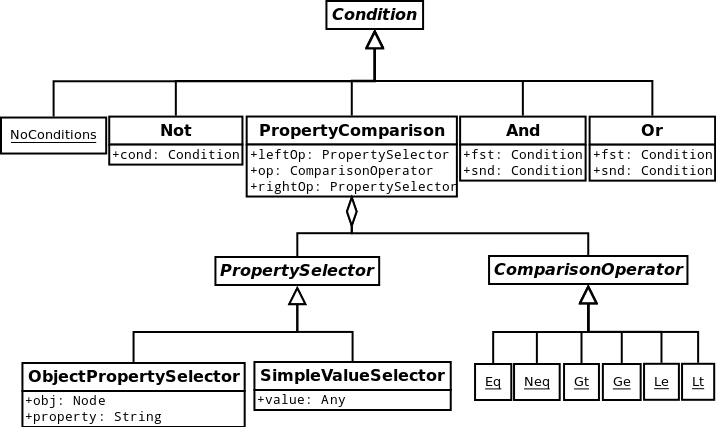
\includegraphics[scale=1]{images/conditions-uml.png}
\end{center}

W makrach można wyszczególnić dwa rodzaje operacji. Są to przechodzenie drzewa składniowego i~wyszukiwanie interesujących wzorców oraz budowanie drzew składniowych wyrażeń, którymi mają być zastąpione znalezione wzorce. Z~tego powodu implementacja makra służącego do transformowania wyrażeń logicznych została podzielona na dwie części realizujące te zadania.

Pierwszą z~nich są tzw. klasy transformujące (ang. Transformers), które zajmują się wyszukiwaniem wzorców w~drzewie i~zamianą ich na docelowe wyrażenia. Drugą -- budowniczy (ang. Builders) zajmujący się tworzeniem drzew składniowych wspomnianych wyrażeń. Odseparowanie tych dwóch czynności oraz wprowadzenie kilku poziomów w~hierarchii klas pozwoliło na stworzenie prostego w~analizie kodu makra. Jest to kluczowe, gdyż mechanizm makr jest sam w~sobie dość skomplikowany.  Ze względu na niewielką objętość kodu pozwoliłem sobie na zamieszczenie implementacji poniżej.

\inputminted{scala}{listings/scala/boolean-macro-implementation.scala}

Jak widać, na poziomie implementacji logiki makra wszystko ogranicza się do wywołań kilku metod poprzedzonych sekcją dopasowywania do wzorca znanego z~języka Scala.

\medskip\noindent Przykładowe użycie stworzonego makra wygląda następująco.

\inputminted{scala}{listings/scala/macro-usage.scala}

W powyższym przykładzie \texttt{nameCondition} oraz  \texttt{nameConditionImplicit} przechowuje poniższą wartość

\inputminted{scala}{listings/scala/macro-usage-result.scala}

\section{Serializacja do języka Cypher}

By zbudowane z~wykorzystaniem NeoDSL zapytania mogły być wykonane przez serwer bazy danych muszą być zamienione na wyrażenia języka Cypher. Podrozdział ten ma na celu opisanie struktur realizujących to zadanie. 

Przypomnijmy, że w~każdym zapytaniu języka Cypher da się wyszczególnić kilka głównych składowych odpowiadających odmiennym zadaniom. Przykładem może być chociażby zapytanie do wyszukiwania danych w~grafie, które składa się z~sekcji \texttt{START}, \texttt{MATCH} oraz \texttt{RETURN}. Te same sekcje pojawiają się również w~innych rodzajach zapytań (jak chociażby w~zapytaniu służącym do aktualizacji danych może pojawić się sekcja \texttt{START}). Z~tego powodu kod służący do serializacji poszczególnych sekcji został podzielony na kilka osobnych obiektów działających w~sposób niezależny. Dzięki temu możliwe jest ponowne jego wykorzystanie w~przypadku implementacji różnych rodzajów zapytań.

\subsection{Struktura}

Głównym obiektem zajmującym się serializacją jest \texttt{CypherSerializer}. Jego zadaniem jest obsługa wszystkich rodzajów zapytań i~delegowanie serializacji do klas odpowiedzialnych za dany typ.

Jedną z~nich jest \texttt{SelectSerializer}, która odpowiada za serializację zapytań typu Select służących do wydobywania danych z~bazy. Realizuje ona swoje zadanie z~wykorzystaniem obiektów odpowiedzialnych za poszczególne sekcje zapytań takie jak: \texttt{StartSerializer}, \texttt{MatchSerializer}, \texttt{ReturnSerializer}, \texttt{WhereSerializer}. Na następnej stronie przedstawiona została graficzna reprezentacja powiązań pomiędzy poszczególnymi klasami.

\newpage

\begin{center}
	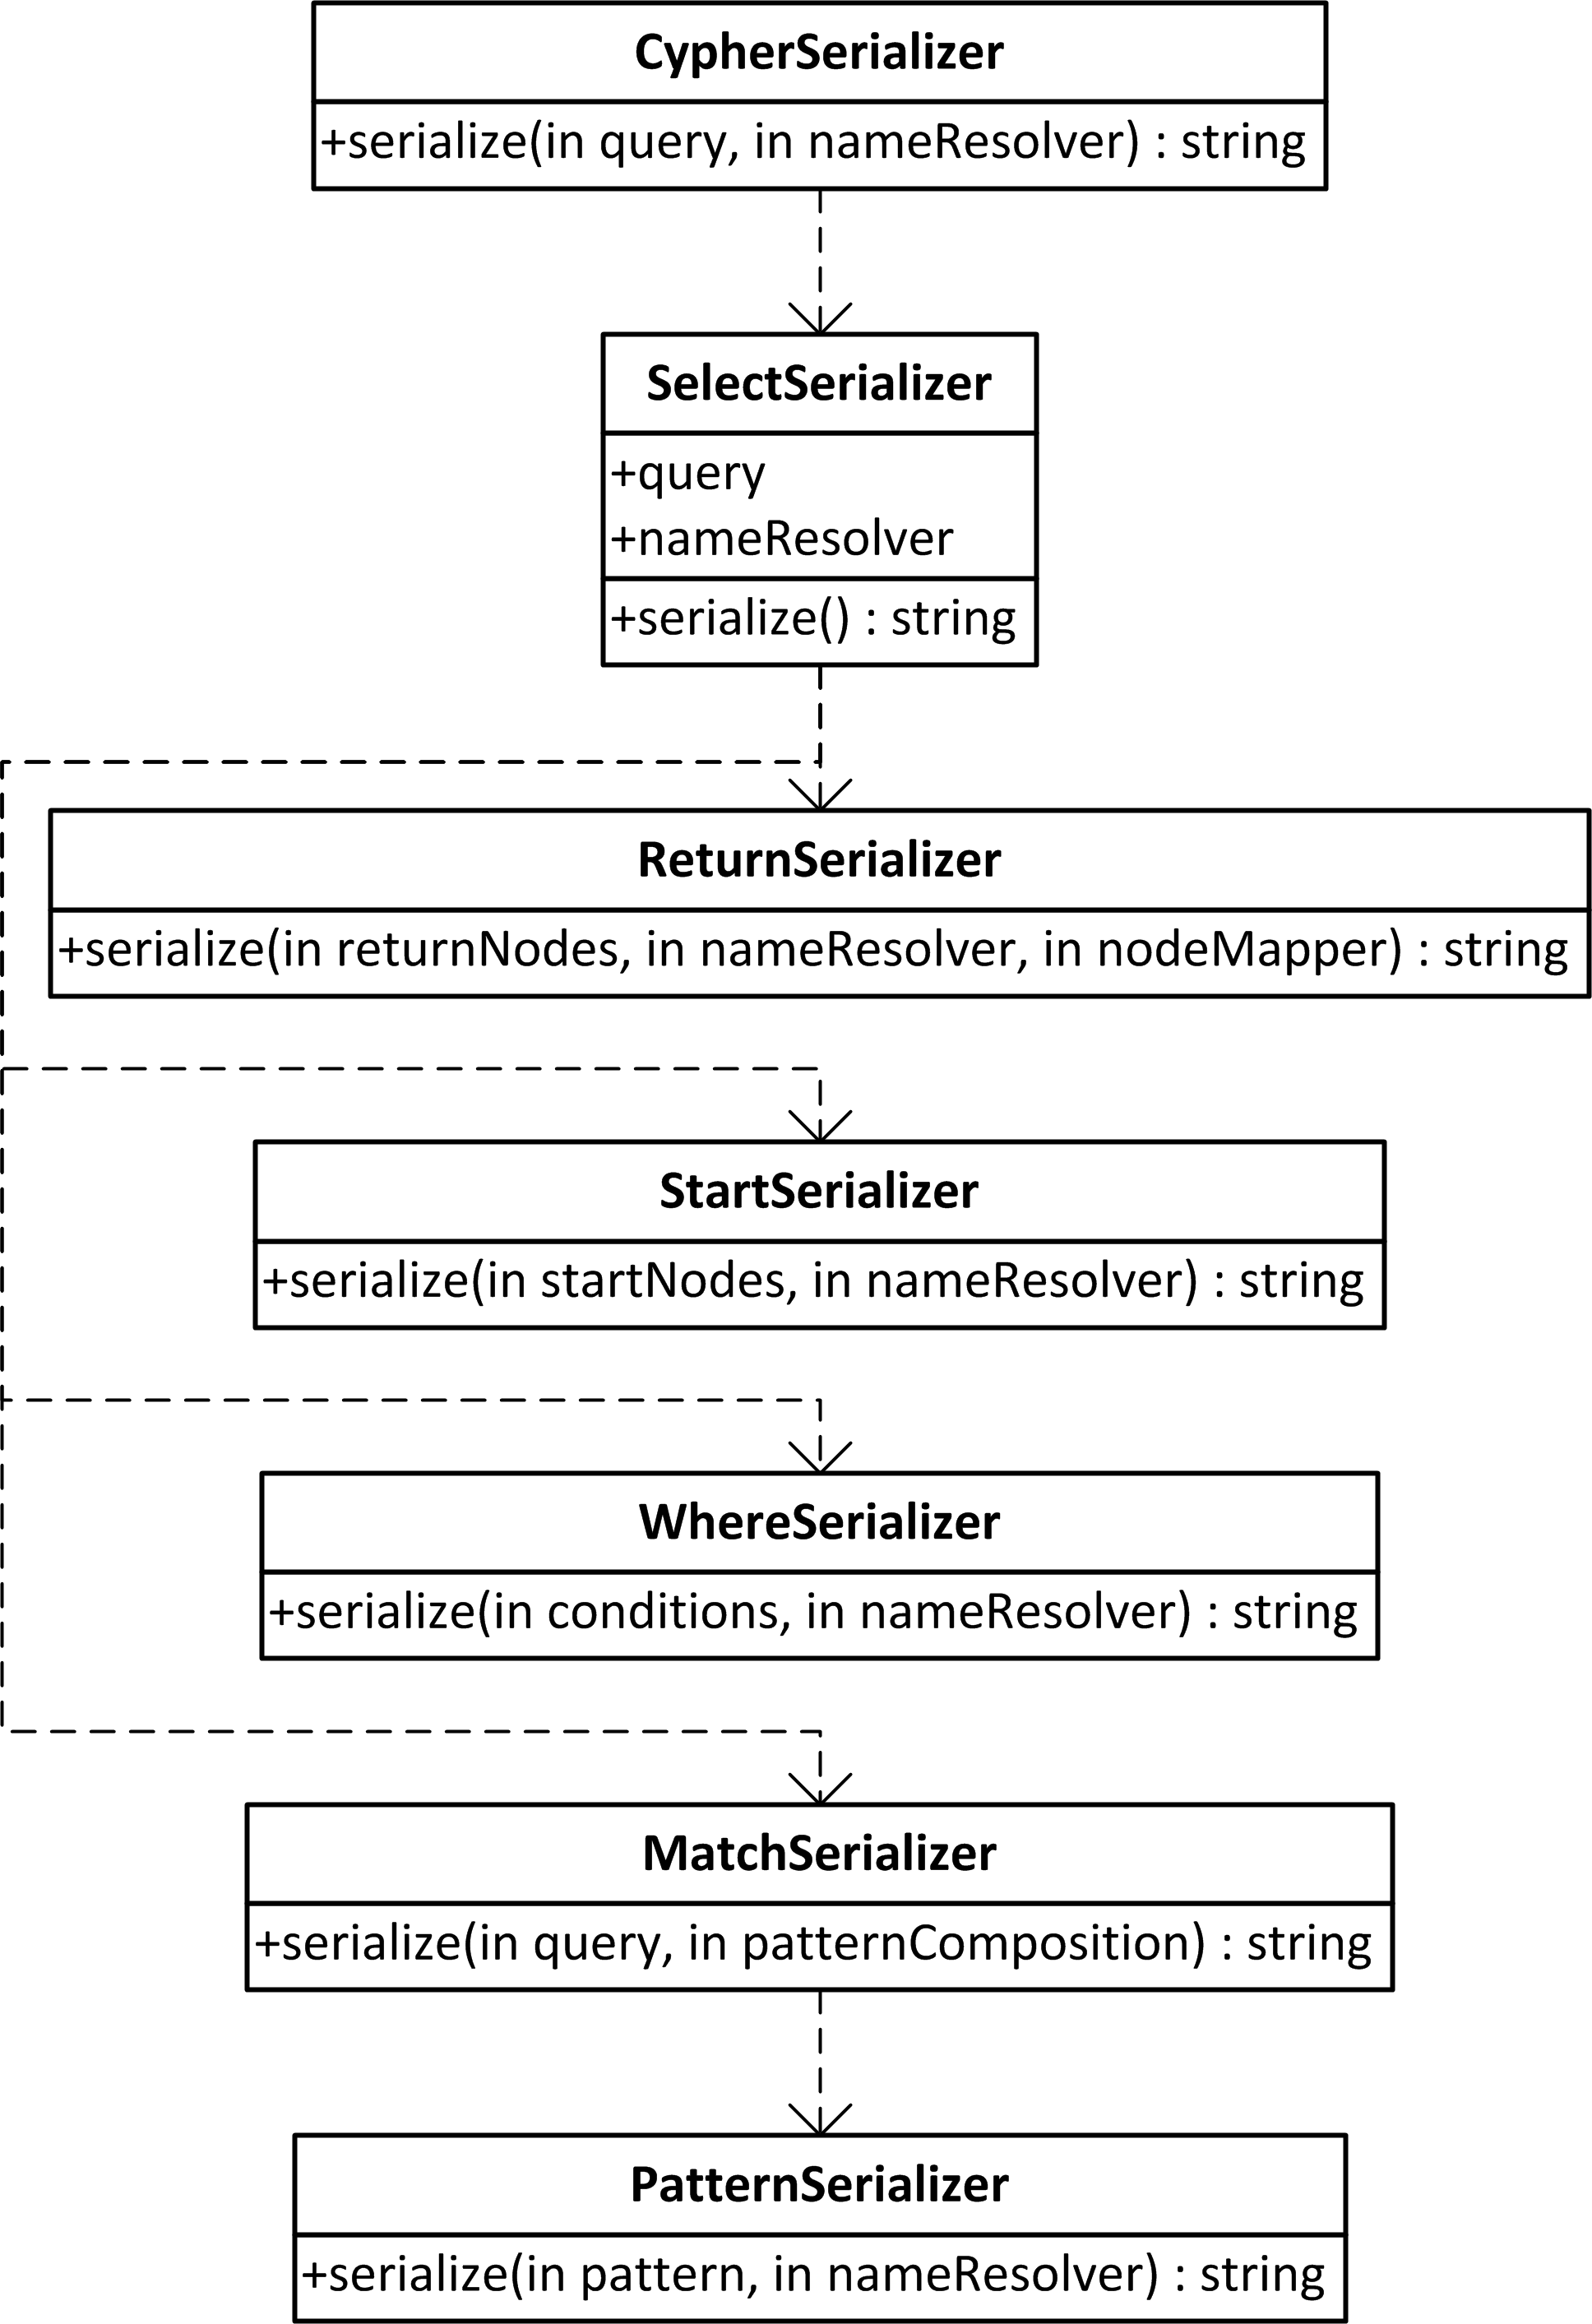
\includegraphics[scale=1]{images/cypher-serialization-uml.png}
\end{center}

\subsection{Uwspólnianie nazw zmiennych}

W zapytaniach języka Cypher węzłom oraz krawędziom nadawane są nazwy służące do odwoływania się do nich w~dalszych częściach zapytania. Ze względu na to, że poszczególne sekcje serializowane są w~sposób niezależny, potrzebny jest mechanizm służący do uwspólniania używanych nazw. Do rozwiązania tego problemu wprowadzony został interfejs \texttt{NameResolver}. Służy on do przydzielania nazw węzłom przekazanym do metody \texttt{name}. Instancja klasy implementującej wspomniany interfejs powinna zawsze zwracać tę samą unikalną nazwę dla każdego przekazanego węzła. Domyślna implementacja, którą jest \texttt{BasicNameResolver} przydziela nazwy według stosownej konwencji. Węzłom pojawiających się w~zapytaniu o~określonym wewnętrznym identyfikatorze przydzielana jest nazwa o~wartości identyfikatora z~prefiksem \texttt{id\_}. Pozostałym węzłom przydzielany jest kolejny wolny numer (zaczynając od 1) z~prefiksem \texttt{n\_}. Przykładowe nazwy to np. \texttt{id\_10} przydzielona dla węzła o~identyfikatorze równym 10 oraz \texttt{n\_2}, która może być przydzielona dowolnemu anonimowemu wierzchołkowi.

\section{Zwracanie wyników}

Istotnym zadaniem narzędzia miało być ukrycie wewnętrznych mechanizmów bazy danych i~danie klientowi złudzenia pracy wyłącznie z~klasami które sam zdefiniował. By osiągnąć ten cel, na poziomie wykonywania zapytań zwracane dane muszą być przetransformowane do klas domenowych. Zadanie zostało zrealizowane z~wykorzystaniem prostego ,,mappera" obiektowego używającego mechanizmu refleksji.

\subsection{Refleksja w~Scali}

Język Scala od wersji 2.10 udostępnia mechanizm refleksji dedykowany do tego języka\cite{scalareflection}. We wcześniejszych wersjach refleksja mogła być realizowana wyłącznie przy pomocy API udostępnianego razem z~językiem Java. Refleksja pozwala na odczytywanie informacji o~dowolnej klasie w~trakcie działania programu. Informacje, jakie można uzyskać to np. zdefiniowane pola, metody czy w~szczególności konstruktory. Poza informacją o~dostępnych polach istnieje również możliwość ich modyfikacji, wywoływania metod czy tworzenia instancji danego typu. Jest to zatem nieodzowny mechanizm stosowany przy implementacji narzędzi tworzących obiekty w~sposób dynamiczny.

Oczywistą wadą refleksji jest mniejsza wydajność niż w~przypadku bezpośredniego operowania na klasie. Na maszynie testowej o~poniższych parametrach został wykonany pomiar porównujący wydajność tworzenia instancji prostych obiektów w~sposób bezpośredni, z~wykorzystaniem refleksji oraz z~refleksją wraz z~mechanizmem pamięci podręcznej.

\begin{tabular}{|l|l|l|l|}
  \hline 
  \textbf{Procesor} & \textbf{Pamięć RAM} & \textbf{Wersja Javy} & \textbf{Rozmiar Sterty} \\
  \hline
  Core 2 Duo 2.4 GHz & 4 GB & 1.7.0\_01 & 1024 MB \\
  \hline
\end{tabular} 

\newpage
Oto wyniki tego pomiaru przedstawiające jak wiele razy refleksja okazała się wolniejsza od bezpośredniego operowania na klasie.

\begin{figure}[H]
	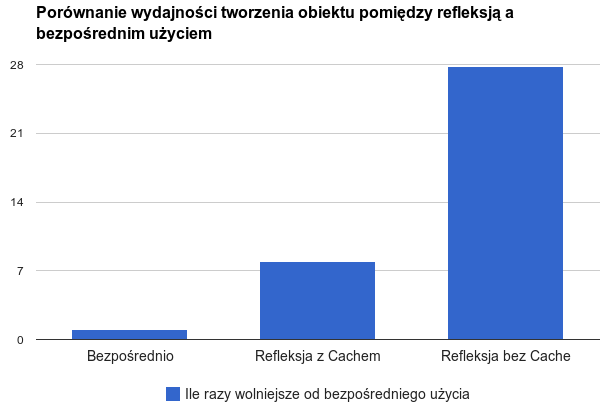
\includegraphics[scale=0.65]{images/reflection-comparison.png}
	\caption{Porównanie wydajnościowe refleksji w~Scali}
	\label{fig:reflection_comparison}
\end{figure}

Z powyższego wykresu wynika iż refleksja w~podstawowym użyciu jest wyraźnie wolniejsza (aż 28 razy) jednak po zastosowaniu mechanizmu pamięci podręcznej wydajność znajduje się na akceptowalnym poziomie.

\subsection{Mapper obiektowy}

Po wykonaniu zapytania, baza danych zwraca wyniki w~określonym przez siebie formacie. Może to być np. format JSON w~przypadku implementacji REST--owej. Oczywiście narzędzia do obsługi bazy Neo4j dostarczają narzędzia do obsługi wyników. Zajmują się one obsługą poszczególnych pól i~rozpoznawaniem typu wartości. NeoDSL również udostępnia tego typu interfejsy mające na celu ujednolicenie dostępu do różnych baz grafowych. Interfejsem opakowującym pojedynczy wynik zapytania jest \texttt{ResultItem}. Zadaniem jego implementacji jest dostarczanie struktury odwzorowania, która dla określonej nazwy pola zwraca jego wartość otrzymaną z~silnika bazy danych. Jedyną dostępną implementacją jest \texttt{Neo4jResultItem} które zajmuje się tłumaczeniem wyników otrzymanych z~serwisu REST.

Silnik obsługujący wybraną bazę grafową powinien implementować interfejs \texttt{ExecutionEngine}. Interfejs ten wymaga by jego implementacja dostarczała metodę \texttt{exec}. Metoda ta powinna dla każdego obsługiwanego przez NeoDSL zapytania zlecać jego wykonanie oraz zwracać wyniki w~postaci kolekcji obiektów typu \texttt{ResultItem}.

Oczywiście \texttt{ResultItem} jest dość ogólnym typem i~nie odpowiada strukturze stworzonej przez programistę wykorzystującego narzędzie. Potrzebny jest zatem mechanizm zajmujący się zamianą obiektów typu \texttt{ResultItem} na instancje klas wybranego typu. Zadanie to realizuje \texttt{ObjectMapper}. Domyślna implementacja tj. \texttt{NodeObjectMapper} wykorzystuje wspomniany już mechanizm refleksji. Tworzy on najpierw instancję danej klasy, a~następnie modyfikuje pola o~takiej samej nazwie jak te, określone w~tablicy haszującej (dostępnej w~obiektach typu \texttt{ResultItem}).

Ze względu na problemy wydajnościowe jakich dostarcza mechanizm refleksji, dla informacji pozyskanych w~sposób dynamiczny wprowadzony został mechanizm pamięci podręcznej.

\chapter{Przykład wykorzystania NeoDSL}

Rozdział ten ma na celu zaprezentowanie kompletnego przykładu zastosowania NeoDSL. Będzie nim społecznościowa zawierająca kilka podstawowych relacji spotykanych w~serwisach społecznościowych.

\subsection{Sieć społecznościowa}

Sieci społecznościowe są idealnym przykładem do prezentowania zalet baz grafowych. Skupiają się one bowiem na relacjach występujących między osobami takimi jak np. znajomość, partnerstwo, które można rozpatrywać na kilku poziomach głębokości. Silniki rekomendacji stosowane w~serwisach społecznościowych dostarczają informacji o~osobach, które użytkownicy mogą znać bazując na powiązaniach znajomych. Proponują one również interesujące strony, informacje w~oparciu gusta osób o~podobnych zainteresowaniach. Implementacja takich zachowań w~bazach grafowych jest niezwykle prosta, a~wyniki uzyskiwane są bardzo krótkim czasie. Oto przykładowy schemat sieci społecznościowej nazywanej dalej ,,NeoSocial".

\newpage
\begin{figure}[H]
        \centering
	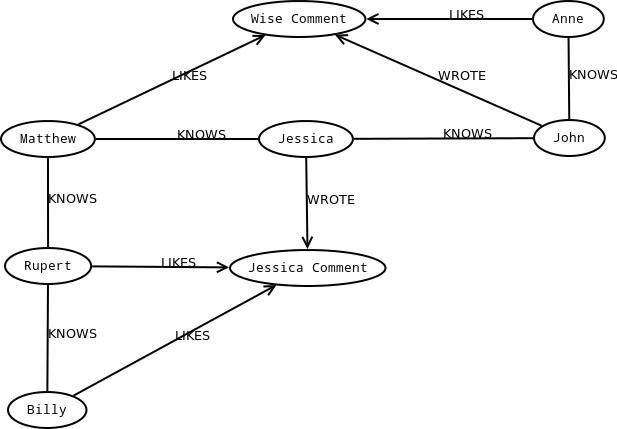
\includegraphics[scale=0.5]{images/socialnetwork-data.png}
	\caption{Przykładowa sieć społecznościowa ,,NeoSocial"}
	\label{fig:neosocial_data}
\end{figure}

Elipsy reprezentują poszczególne węzły, napis w~ich wnętrzu odpowiada imieniu osoby lub treści komentarza napisanego przez jednego z~użytkowników. Wierzchołki połączone są następującymi krawędziami  ,,KNOWS" -- służy do modelowania relacji ,,znajomości" pomiędzy osobami, ,,WROTE" -- wskazuje autora komentarza oraz ,,LIKES" -- łączy osoby z~komentarzami dla których wyrażają one aprobatę.

Aby odwzorować powyższą strukturę w~NeoDSL potrzebne jest utworzenie klasy \texttt{Person} do reprezentowania osób. Zawierać ona będzie pole \texttt{name} odpowiadające imieniu oraz pola odpowiadające relacjom w~jakich może znajdować się osoba. Są to \texttt{knows} oraz \texttt{likes}. Do odwzorowania komentarzy służyć będzie klasa \texttt{Comment}. Składa się ona z~pola \texttt{content} przechowującego treść wpisu oraz krawędzi \texttt{writtenBy}. Pełny fragment kodu znajduje się poniżej.

\inputminted{scala}{listings/scala/examples/socialnetwork/domain-classes.scala}

\subsection{Zapytania w~sieci społecznościowej}

Zapytania związane z~osobami zostaną zdefiniowane w~ramach obiektu \texttt{Person} (W Scali jest to tzw. obiekt stowarzyszony z~klasą \texttt{Person}, o~jego metodach można myśleć jak o~statycznych metodach klasy \texttt{Person}).

Poniżej przedstawione jedno z~prostszych zapytań służących do wydobywania znajomych danej osoby.

\inputminted{scala}{listings/scala/examples/socialnetwork/person-friends-query.scala}

Ciekawszym i~często używanym przykładem w~kontekście baz grafowych jest zapytanie służące do wyszukiwania znajomych znajomych danej osoby. Może być ono użyte przy implementacji silnika rekomendacji znajomych. Oto ono zdefiniowane przy pomocy NeoDSL.

\newpage

\inputminted{scala}{listings/scala/examples/socialnetwork/person-fof-query.scala}

Uruchomienie powyższego zapytania z~argumentem reprezentującym wierzchołek ,,Jessica" zwróci węzły ,,Anne" oraz ,,Rupert" (por. \ref{fig:neosocial_data}).

\inputminted{scala}{listings/scala/examples/socialnetwork/person-fof-result.scala}
\inputminted{text}{listings/text/person-fof-result.txt}

Zaprezentowane dotychczas przykłady operowały wyłącznie na jednym typie krawędzi, oczywiście możliwe jest również mieszanie różnych rodzajów w ramach pojedynczych wzorców. Poniższe zapytanie służy do wyszukiwania znajomych, którzy ,,polubili" komentarz o wybranej treści.

\inputminted{scala}{listings/scala/examples/socialnetwork/friendswholikecomment.scala}

Jego uruchomienie dla węzła John oraz komentarza ,,Wise Comment" zwraca pojedynczą parę obiektów reprezentujących wierzchołek ,,Anne" oraz wspomniany komentarz.

\inputminted{scala}{listings/scala/examples/socialnetwork/friendswholikecomment-exec.scala}
\inputminted{text}{listings/text/friendswholikecomment-result.txt}

\chapter{Potencjalne funkcjonalności NeoDSL}

Obecna funkcjonalność NeoDSL obejmuje przeszukiwanie bazy danych. Możliwy jest jednak dalszy rozwój tego narzędzia. W~rozdziale zostaną opisane niektóre z~możliwych do zaimplementowania usprawnień wraz z~proponowanym sposobem implementacji.

\section{Aktualizacja danych}

Jednym z~istotnych rozszerzeń byłoby dodanie możliwości aktualizowania i~wstawiania danych. Aktualnie, możliwe jest jedynie przeszukiwanie bazy bez jakiejkolwiek możliwości zmian jej stanu. 

Osiągnięcie tego celu możliwe byłoby z~wykorzystaniem istniejących już struktur. Budowanie wzorców nie wymagałoby praktycznie żadnej zmiany, a~jedynym istotnym elementem byłaby implementacja zapytań oraz ich serializacja do języka Cypher. Poniżej przedstawiono przykład potencjalnej implementacji.

\inputminted{scala}{listings/scala/missing-features-update.scala}

\section{Sortowanie oraz dodatkowe ograniczenia na wyniki}

Obecnie możliwe jest definiowanie prostych ograniczeń na zwracane wyniki (jak porównanie wartości pól węzłów). Nie ma natomiast możliwości wyrażenia wymogu unikatowości zwracanych wyników czy też określania kolejności w~jakiej będą one przekazywane. Oczywiście mowa tutaj o~wyrażaniu tych ograniczeń w~taki sposób, aby mogły być one zrealizowane przez serwer bazy danych. Nic nie stoi na przeszkodzie aby spełnić je po stronie klienta korzystając ze standardowych funkcjonalności kolekcji języka Scala.

Implementacja tego typu zachowań mogłaby też zostać zrealizowana w~podobny sposób, w~jaki możliwe jest nakładanie warunków na pola zwracanych węzłów tj. z~wykorzystaniem makr. Konieczna byłaby wówczas analiza wyrażeń, które służą np. do wskazania pola po jakim powinno odbywać się sortowanie. 

\medskip\noindent Poniżej przykład tego w~jaki sposób mogłoby wyglądać wykorzystanie mechanizmu.

\inputminted{scala}{listings/scala/missing-query-features.scala}

% zakończenie 
\summary

Popularyzacja języków takich jak Scala skłania do poszukiwania efektywniejszych i~wygodniejszych w obsłudze narzędzi do baz danych. Projekty takie jak Squeryl czy Rogue pokazują olbrzymi potencjał drzemiący językach dziedzinowych. Ich stosowanie pozwala na wyrażanie zapytań w równie intuicyjny sposób jak możliwe jest to z wykorzystaniem np. SQL-a, dając dodatkowo funkcjonalności takie jak sprawdzanie poprawności wyrażeń na etapie kompilacji i~automatyczne mapowanie wyników na obiekty.

Bazy grafowe stanowią natomiast świeże spojrzenie na problem składowania danych. Reprezentacja grafowa dużo bardziej odpowiada rzeczywistości, którą programiści modelują w~swoich aplikacjach. W~coraz większym stopniu mamy do czynienia z~danymi, które powiązane są wieloma zależnościami. Neo4j jak i~inne bazy grafowe stanowią wydajne rozwiązanie dla tego typu zastosowań.

Powstały w ramach pracy język dziedzinowy był eksperymentem mającym na celu odkrycie ciekawych technik pomocnych przy ich definiowaniu. Jedną z nich jest np. zastosowanie makr języka Scala. Okazuje się, że mechanizm ten może być niezwykle użyteczny i pozwala na osiągnięcie spektakularnych efektów. Zastosowanie tego mechanizmu w NeoDSL pozwoliło na wyrażanie warunków logicznych z wykorzystaniem standardowej składni Scali. Podobne efekty osiągane w~innych narzędziach z wykorzystaniem odmiennych technik niejednokrotnie prowadzą do trudnego w~analizie kodu opartego na sztuczkach programistycznych. Jak się jednak okazuje, przy właściwym wykorzystaniu makr można stworzyć prostą i~czytelną implementację.

Niewątpliwie, potencjał drzemiący w~językach dziedzinowych jest ogromny, a~zastosowanie ich w~przypadku baz danych jest tylko jednym z~wielu. Ciekawymi zastosowaniami DSL-i może być np. język: do definiowania interfejsu użytkownika, budowania XML czy też pisania testów w~formie specyfikacji, która podlega weryfikacji.

% załączniki (opcjonalnie):
\appendix
\chapter{Zmiany w~Neo4j 2.0 względem 1.x}

Stworzone narzędzie było projektowane z~myślą o~Neo4j w~wersji 1.9.x, która w~momencie pisania większej części pracy była obowiązującym stabilnym wydaniem. Wersja druga, przyniosła znaczące zmiany, które wymagają omówienia (stoją one w~sprzeczności z~częścią opisanych tu mechanizmów).

Jedną z~bardziej istotnych zmian jest tak zwany mechanizm etykietowania, który pozwala na grupowanie węzłów. Poza możliwością określenia typu każdego węzła możliwe stało się nakładanie tzw. więzów (ang. Constraints) na określone typy. Pozwala to na definiowanie schematu bazy. Pojawienie się mechanizmu etykiet miało również wpływ na rozszerzenie języka Cypher. Możliwe jest np. wyszukiwanie wzorców z~węzłami określonego typu.

Kolejnym mechanizmem który został gruntownie przebudowany jest indeksowanie. W~przypadku wydań z~serii 1.x narzut związany z~obsługą indeksowania był zrzucony na programistę. W~dodatku by wykorzystać dany indeks w~zapytaniu trzeba było zażądać tego w~sposób jawny w~sekcji \texttt{START}. Obecnie, indeksy przypominają w~dużo większym stopniu funkcjonalność znaną z~baz relacyjnych. Nie ma potrzeby jawnego określania jaki indeks powinien zostać wykorzystany w~zapytaniu, natomiast samo zarządzanie nimi stało się możliwe z~poziomu języka Cypher.

Zmiany dotknęły również języka Cypher który jak określają twórcy stał się jeszcze bardziej deklaratywny. Istotną nowością jest np. opcjonalność sekcji \texttt{START}. Zapytania nie muszą zawierać jakichkolwiek węzłów początkowych niemniej zalecane jest ograniczanie zbioru węzłów, po których odbywać będzie się wyszukiwanie. Pozostałe zmiany miały na celu uproszczenie składni.

% literatura (obowiązkowo):
\bibliographystyle{unsrt}
\bibliography{master-thesis}

% spis tabel (jeżeli jest potrzebny):
\listoftables

% spis rysunków (jeżeli jest potrzebny):
\listoffigures

\oswiadczenie

\end{document}
